% !TEX encoding = UTF-8 Unicode
% !TEX root = ../rapport.tex

\chapter{Introduction}\label{intro}

Les réseaux sans fil font depuis plus d'une dizaine d'années partie intégrante de la vie quotidienne des entreprises, des particuliers, de l'industrie et d'autres organisations. Ils
représentent aujourd'hui une des briques de base sur lesquelles vont se fonder les systèmes
intelligents omniprésents qui vont constituer une des technologies de l'avenir. Cependant, la majeure partie de ces technologies sans fils, à commencer par le Wifi, elle est basée  sur des infrastructures fixes, limitant la mobilité des utilisateurs. Pour faciliter cette mobilité, il existe  un autre type de réseau, de plus en plus courant, qui  permet aux nœuds du réseau de communiquer directement entre eux sans nécessiter d’infrastructure : ce sont les réseaux ad hoc.

On distingue donc deux principales classes de réseaux sans fils, les classiques structurés et les non structurés comme les réseaux ad hoc. Les réseaux ad hoc offrent la possibilité de connecter différents dispositifs sans avoir à préinstaller une infrastructure fixe comme dans les réseaux traditionnels. Dans les réseaux ad hoc, l’ensemble des nœuds communiquent directement entre eux (voir figure \ref{reseauAdHoc}). Nous nous allons nous intéresser un des types particulier des réseaux ad hoc on nommera les (WSN, VANET, VSN) qui seront expliqués plus en détail dans ce qui suit.

\begin{figure}[h]
\centering
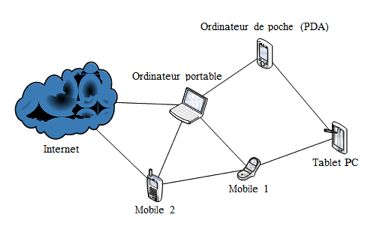
\includegraphics[scale=0.8]{intro/reseauAdHoc.png}
\caption{\label{reseauAdHoc} Réseau ad hoc}
\end{figure}


\section{Les capteurs}

On dénombre de types de capteurs :
\renewcommand\labelitemi{\textbullet}
\begin{itemize}

\item \textbf{Model de mesure :} un capteur est un dispositif équipé de fonctionnalités de sensation avancées. Il mesure ou détecte un événement réel, comme le mouvement, la chaleur ou la lumière et convertit la valeur mesurée dans une représentation analogique ou numérique. Il prélève des informations et élabore à partir d’une grandeur physique (information d’entrée), une autre grandeur physique de nature électrique.

\item \textbf{Capteur intelligent :} Les capteurs intelligents (Smart Sensors) sont des dispositifs matériels dans lesquels coexistent le(s) capteur(s) et les circuits de traitement et de communication. Leurs relations avec des couches de traitement supérieures vont bien au-delà d’une simple « transduction de signal ». Les capteurs intelligents sont des « capteurs d’informations » et non pas simplement des capteurs et des circuits de traitement du signal juxtaposés. De plus, les « Smart Sensors » ne sont pas des dispositifs banalisés car chacun de leurs constituants a été conçu dans l’objectif d’une application bien spécifique.

\end{itemize}

En résumé les capteurs sont des petits entités électroniques à faible coût qui ont pour but de récolter des informations de leurs environnement proches comme la température, la vitesse, le bruit, la pression… et éventuellement de les traiter.

 Un capteur intelligent contient quatre unités de base (voir Figure \ref{archiCapteur}). :
 \begin{itemize}

\item \textbf{L'unité d’acquisition :} composée d’un capteur qui obtient des mesures sur les paramètres environnementaux et d’un convertisseur Analogique/Numérique qui convertit l’information relevée et la transmet à l’unité de traitement.

\item \textbf{L'unité de traitement :} composée d’un processeur et d’une mémoire intégrant un système d’exploitation spécifique. Cette unité possède deux interfaces, une interface pour l’unité d’acquisition et une interface pour l’unité de communication. Elle acquiert les informations en provenance de l’unité d’acquisition et les envoie à l’unité de communication. Cette unité est chargée aussi d’exécuter les protocoles de communications qui permettent de faire collaborer le capteur avec d’autres capteurs. Elle peut aussi analyser les données captées.

\item \textbf{L'unité de communication : } unité responsable de toutes les émissions et réceptions de données via un support de communication radio. Elle peut être de type optique, ou de type radiofréquence.

\item \textbf{L'unité de contrôle d'énergie (batterie) :} un capteur est muni d’une batterie pour alimenter tous ses composants. Cependant, à cause de sa taille réduite, la batterie dont il dispose est limitée et généralement irremplaçable. Pour cela, l’énergie est la ressource la plus précieuse puisqu’elle influe directement sur la durée de vie des capteurs.

\end{itemize}

Selon le domaine d'application, il peut aussi contenir des modules supplémentaires comme le système de positionnement GPS (Global Positioning System) et un mobilisateur lui permettant le déplacement.

\begin{figure}[h]
\centering
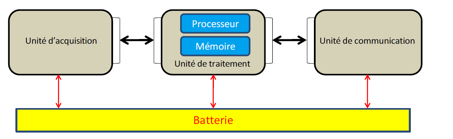
\includegraphics[scale=0.8]{intro/archiCapteur}
\caption{\label{archiCapteur} Architecture d’un capteur}
\end{figure}


\section{Caractéristiques principales d’un capteur}
Deux entités sont fondamentales dans le fonctionnement d’un capteur : l’unité d’acquisition qui est le cœur physique permettant la prise de mesure et l’unité de communication qui réalise la transmission de celle-ci  vers d’autres dispositifs électroniques. Ainsi, fonctionnellement chaque capteur  possède un rayon de communication (Rc) et un rayon de sensation (Rs).  La  Figure \ref{percept} montre les zones définies par ces deux rayons pour le capteur A. La zone de communication est la zone où le capteur A peut communiquer avec les autres capteurs (le capteur B dans la Figure \ref{percept}). D’autre part, la zone de sensation est la zone où le capteur A peut capter l’événement.

\begin{figure}[h]
\centering
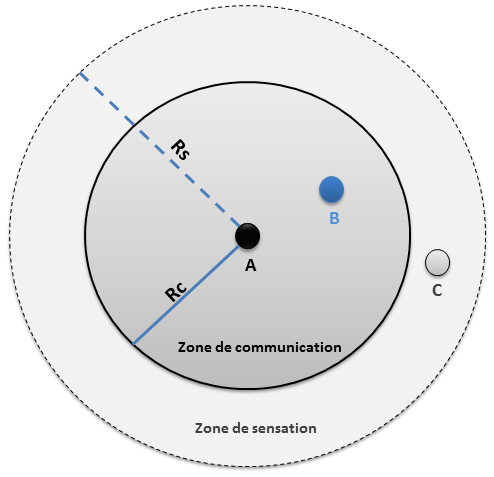
\includegraphics[scale=0.8]{intro/percept}
\caption{\label{percept} Rayon de communication et de sensation}
\end{figure}

Pour qu’un capteur ait une portée de communication suffisamment grande, il est nécessaire d’utiliser un signal  assez puissant. Cependant, l’énergie consommée serait importante. Il existe dans le monde plusieurs fabricants de capteurs Crossbow, Cisco, Dalsa, EuroTherm, et Sens2B. Parmi ces capteurs, il existe quelques-uns qui sont capables de varier la puissance du signal émis afin d’élargir/réduire le rayon de communication et en conséquence la zone de communication. La  Figure \ref{imageCapteur}  montre un capteur sans fil.

\begin{figure}[h]
\centering
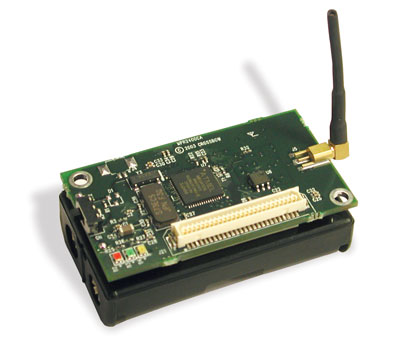
\includegraphics[scale=0.8]{intro/imageCapteur}
\caption{\label{imageCapteur} Capteur sans fil}
\end{figure}


\section{Caractéristiques des capteurs actuels}
Nous voyons donc rapidement les contraintes que vont rencontrer les capteurs :
\begin{itemize}

\item \textbf{Une faible puissance de calcul} : quand les PCs nouvelle génération peuvent avoir jusqu’à4 processeurs, chacun cadencé à 3GHz, ou quand les derniers Smartphones peuvent fonctionner jusqu’à 800MHz, un capteur actuel est à peine plus puissant qu’une calculatrice graphique produite dans les années 90.

\item \textbf{Un espace de stockage mémoire limité} de quelques kilos à quelques mégaoctets nécessite des algorithmes distribués, localisés et collaboratifs.

\item \textbf{Une puissance radio limitée} : l’ordre de grandeur des portées actuellement atteignables par les principaux capteurs est d’une centaine de mètres en extérieur et de quelques dizaines de mètres en intérieur. Cette portée est largement dépendante de la fréquence utilisée et de l’environnement. Elle nécessite un routage multi-saut pour l’acheminement des données vers une entité de collecte, le puits : les capteurs ne peuvent communiquer qu’avec les capteurs de leur voisinage direct qui vont relayer les communications.

\item \textbf{Un débit faible} : les composants radio d’un capteur sont limités à quelques centaines de kilo-octets par seconde.

\item \textbf{Une réserve d’énergie réduite} : même s’il existe des mécanismes de recharge d’énergie, la durée de vie d’un capteur reste directement liée au niveau de sa batterie. Cette réserve d’énergie est partagée par chaque unité d’un capteur mais l’unité de communication va en consommer près de 95\% lors du fonctionnement actif du capteur. Il est donc naturel qu’une forte recherche s’effectue à la fois sur l’augmentation des capacités des batteries, sur les dispositifs de transmission radio ultra-basse consommation, les architectures basse consommation, et enfin, sur les mécanismes d’endormissement et sur des protocoles de communication spécifique.

\end{itemize}

De par leurs contraintes On doit donc bien comprendre que la force d’un réseau de capteurs ne tient pas à la qualité des capteurs individuellement mais à leur collaboration : l’ensemble du réseau est supérieur à la somme des capteurs qui le composent. Cette collaboration est possible grâce à des protocoles.


\section{Exemple d’application des capteurs}
Dans cette partie nous aller présenter quelque exemple d’application des capteurs.
\begin{itemize}

\item \textbf{capteurs de mesures physiques} : pression force accélération, position,température champ magnétique, radioactivité, débit (liquide ou gaz).

\item \textbf{capteurs chimiques} : humidité relative de l'air, capteurs de gaz, capteurs électrochimiques, biocapteurs

\item \textbf{capteurs multimédia} : capteurs optiques et d'image, son

\item \textbf{applications médicales} : mesures d'impédance, instrumentation ambulatoire imagerie médicale, tomographie-imagerie, dermatologie, post urologie, tissus biologiques

\item \textbf{capteurs pour l'automobile} : contrôle de combustion, sécurité et aide au pilotage le pilotage assisté, hypovigilance et sécurité, gadgets contemporains.

\item \textbf{capteurs pour la climatologie} : capteurs de pluie, les capteurs de vent, capteurs d'ensoleillement.

\end{itemize}


\section{Réseau de capteur sans fil (Wireless sensors network)}
Les réseaux de capteurs sans fil  WSN  sont un type particulier de réseau Ad-hoc .Ces réseaux sont formés d’une multitude de petits dispositifs autonomes, capables de s’auto-organiser pour communiquer entre eux via des liens radio, et ainsi travailler pour la collecte, le partage et le traitement coopératif des informations sur leur environnement, le tout sans intervention humaine. Ces dispositifs sont peu coûteux, mais peu performants, et peuvent être utilisés en masse sans prendre soin de s’occuper de chacun d’eux. Dans un tel réseau, chaque nœud est un dispositif électronique qui possède une capacité de calcul, de stockage, de communication et d’énergie. Ils sont l’ultime signe actuel de l’informatisation de masse et du besoin absolu de réseautage (Networking) Un  exemple de réseaux de capteurs est fourni  dans la  (Figure \ref{WSN}).

\begin{figure}[h]
\centering
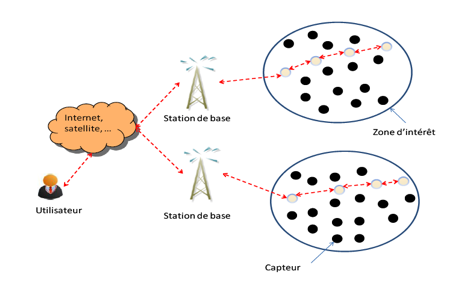
\includegraphics[scale=0.8]{intro/WSN}
\caption{\label{WSN} Réseaux de capteurs}
\end{figure}


\subsection{Fonctionnement}
Les capteurs sont déployés d’une manière aléatoire dans une zone d’intérêt, et une station de base, située à l’extrémité de cette zone, est chargée de récupérer les données collectées par les capteurs. Lorsqu’un capteur détecte un événement pertinent, un message d’alerte est envoyé à la station de base par le biais d’une  communication entre les capteurs. Les données collectées sont traitées et analysées par des machines puissantes. Les  réseaux de capteurs viennent  en  soutien  de l’environnement et de l’industrie grâce aux récents développements réalisés dans le domaine  des techniques sans  fils.  Depuis  quelques décennies, le besoin d’observer et de contrôler des phénomènes physiques tels que la température, la pression ou encore la  luminosité  est essentiel pour de nombreuses applications industrielles et scientifiques.


\subsection{Architecture d’un réseau de capteurs sans fil}

\begin{figure}[h]
\centering
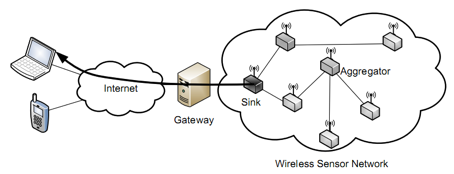
\includegraphics[scale=0.8]{intro/archiWSN}
\caption{\label{archiWSN} architecture d’un réseau WSN}
\end{figure}

La  Figure \ref{archiWSN} représente l’architecture habituelle des réseaux de capteurs sans fils. Ils sont construits autour des quatre principales entités suivantes :

\begin{itemize}

\item \textbf{Le capteur (sensor)} : décrit précédemment.

\item \textbf{L’agrégateur (aggregator)} : Il est en charge d’agréger les messages qu’il reçoit de plusieurs capteurs puis de les envoyer en un seul message au puits (sink). Cette opération a pour principal but de limiter le trafic sur le réseau et donc de prolonger la durée de vie globale du réseau de capteur. Il correspond généralement à la tête d’une grappe (cluster head).

\item \textbf{Le puits (sink)} : Le puits est le nœud final  du réseau. C’est à lui qu’est  envoyé l’ensemble des valeurs mesurées par le réseau.  Il peut arriver qu’il y’ait plusieurs puits sur un  même réseau de capteurs.

\item \textbf{La passerelle (gateway)} : La passerelle est un dispositif qui a la particularité d’avoir deux interfaces réseau. Il permet de relier le réseau de capteurs  sans fils  à un réseau plus traditionnel, typiquement l’internet.   
En effet, habituellement  le réseau de capteurs  ne sert  qu’à  faire remonter les 
mesures, les applications traitant ces informations étant exécutées sur la machine 
de l’utilisateur final.

\end{itemize}


\subsection{Caractéristiques}
Les caractéristiques particulières des WSN modifient les critères de performances par rapport aux réseaux sans fil traditionnels. Dans les réseaux locaux filaires ou les réseaux cellulaires, les critères les plus pertinents sont le débit, la latence et la qualité de service car les nouvelles Activités telles que le transfert d’images,  le  transfert de vidéos, et la navigation sur Internet requièrent un débit important, une faible latence, et une bonne qualité de service. En revanche, dans les réseaux de capteurs conçus pour surveiller une zone d’intérêt,  la longévité du réseau est fondamentale. De ce fait, la conservation de l’énergie est devenue un critère de performance prépondérant et se pose en premier lieu tandis que les autres critères comme le débit ou l’utilisation de la bande passante sont devenus secondaires. Nous verrons dans ce qui suit quelque caractéristique des WSN.

\begin{itemize}

\item \textbf{Absence d’infrastructure} : d’absence d’infrastructure préexistante et de tout genre d’administration centralisée.

\item \textbf{Interférences} : les liens radio ne sont pas isolés, deux transmissions simultanées sur une même fréquence, ou utilisant des fréquences proches, peuvent interférer.

\item \textbf{Taille importante} : un réseau de capteurs peut contenir des milliers de nœuds.

\item \textbf{Hétérogénéité des nœuds} : plusieurs types différents connectant entre eux.

\item \textbf{Topologie dynamique} : les capteurs peuvent être attachés à des objets mobiles qui se déplacent d’une façon libre et arbitraire rendant ainsi la topologie du réseau fréquemment changeante.

\item \textbf{Contrainte d’énergie} : la caractéristique la plus critique dans les réseaux de capteurs est la modestie de ses ressources énergétiques (batterie).

\item \textbf{La capacité de stockage et la puissance de calcul} sont limitées dans un capteur.

\item \textbf{sécurité physique limitée} : Cela se justifie par les contraintes et limitations physiques.

\item \textbf{bande passante limitée} : la bande passante réservée à un nœud est limitée.

\item \textbf{Le faible coût du matériel} : Ce qui facilite une redondance des liens pour assurer une connexité du réseau en cas de panne d’un ou plusieurs capteurs

\end{itemize}

Une des forces d’un réseau de capteurs est sa capacité à être déployé rapidement dans des conditions difficiles. Le Positionnement des nœuds est donc aléatoire. Ces conditions de déploiement conduisent à des contraintes supplémentaires :

\begin{itemize}

\item \textbf{L’impossibilité de remplacer manuellement les nœuds} : pour position inconnu.

\item \textbf{Méconnaissance globale de la topologie du réseau} : due une forte densité et une forte cardinalité du réseau.

\end{itemize}


\subsection{Application des WSN}
Le fort potentiel d’application des réseaux de capteurs en fait un domaine de recherche très actif. Ces dernières années ont vu le passage d’applications anecdotiques à de véritables applications à large échelle. La réduction de plus en plus importante de la taille des capteurs, leur coût de plus en plus faible, ainsi que l’étendue du type de capteurs disponibles (thermique, optique, cinétique, chimique, etc.), permettent aux réseaux de capteurs d’envahir de très nombreux domaines d’application.

On dénombre 3 grandes familles d’applications pour réseaux de capteurs :
\begin{itemize}

\item \textbf{le relevé d’informations} : dans lequel chaque capteur collecte simplement les données et les envoie périodiquement au puits.

\item \textbf{la détection d’événements} : où chaque nœud décide s’il envoie des données au puits en fonction des données qu’il a collectées. Cette décision peut nécessiter au capteur un dialogue avec son voisinage.

\item \textbf{le contrôle intelligent} : dans lequel chaque capteur collecte différentes sortes de données, échange ses informations à travers le réseau et collabore pour former une description de l’état de l’objet ciblé.

\end{itemize}

Il a également été définit un ensemble de scénarios viables visé par les réseaux de capteurs

\begin{itemize}

\item Supervision de l'habitat écologique
\item Surveillance militaire et traque de cibles
\item Supervision des structures et des phénomènes liés à l’environnement (séisme, volcan)
\item Détection en réseau dans l'industrie et le commerce
\item Bâtiment intelligent
\item Domotique
\item Surveillance de l’environnement (volcan, météo…)
\item Santé  (La surveillance des fonctions vitales d'un organisme vivant)
\item Sécurité industrielle et Domestique

\end{itemize}


\subsection{Problématique et Défis}
Les perspectives d’application des réseaux de capteurs sont enthousiasmantes mais les défis qu’elles posent n’en sont pas moins nombreux et complexes. Parmi les problématiques cruciales, nous pouvons citer :
\begin{itemize}

\item \textbf{L’énergie} : cette contrainte impose de concevoir des protocoles économes en énergie.

\item \textbf{Le routage} : Le problème de routage consiste à déterminer un acheminement optimal des paquets à travers le réseau au sens d’un certain critère de performance (Energie par exemple).

\item \textbf{Sécurité} : La puissance de calcul limité des entités d’un capteur ouvre de véritables défis pour concevoir des algorithmes de cryptages distribués et des politiques de confiance spécifiques.

\item \textbf{La collecte de données} : récupérer les données des capteurs et les assemblés.

\item \textbf{Auto-configuration} : Une partie des applications visée appartient au domaine des applications domestiques. Il est donc important que le routage, l’intégration et l’adaptation à l’environnement soient transparents pour l’utilisateur.

\item \textbf{Autoréparation} : Nous venons de le voir, les capteurs sont parfois inaccessibles (intégrés dans un mur, installés chez un particulier, déployés dans une zone dangereuse, etc.) et parfois de conception peu sûre (faible coût de production). Une solution complète doit donc gérer efficacement la perte ou l’ajout d’un nœud dans son réseau.

\item \textbf{Localisation} : Il s’agit de concevoir des mécanismes de localisation réalistes vis-à-vis des contraintes et des applications propres aux réseaux de capteurs. Les solutions actuellement proposées reposent sur des solutions, soit imprécises, soit coûteuses en énergie ou en matériel.

\end{itemize}


